\chapter{Kravspecifikation}

\textbf{Versionshistorik}
\begin{longtabu} to \linewidth{@{}l l l X[j]@{}}
    Version &    Dato &    Ansvarlig &    Beskrivelse\\[-1ex]
    \midrule
    1.0		&	23-09-2015 &		Alle	&	Første udkast til Use Cases. I alt 4, hvor en af funktionaliteterne var, at man kunne optage en lydsekvens\\[-1ex]
    1.1		&	29-09-2015	&	Alle	&	Ændring af Use Cases efter møde med Peter. I alt 5, hvor funktionaliteterne kun dækker over de opstillede krav til projektet. \\[-1ex]
    1.2		&	30-09-2015	&	Alle	&	Små ændring af formuleringerne samt byttet om på UC1 og UC2 og tilføjet en UC6. De ikke-funktionelle krav er blevet tilføjet. Klar til Review\\[-1ex]	
    2.0		&	08-10-2015	& Alle		&	Rettelser efter review møde\\[-1ex] 
    2.1		&	04-11-2015	& Alle		&	Tilføjet Tryktransducer som en sekundæraktør \\[-1ex]

\label{version_Systemark}
\end{longtabu}

\section{Indledning}
Kravspecifikationen vil gennem seks Use Cases beskrive blodtryksmålerens funktionelle krav. Systemets ikke-funktionelle krav er udarbejdet på baggrund af (F)URPS+. Dertil vil der være aktør-kontekst- og Use Casesdiagram samt beskrivelse af de forskellige aktører, der interagerer med systemet.  

\section{Systembeskrivelse}
 Systemet skal kunne vise et blodtryksignal kontinuert i en graf. Derudover skal systemet kunne kalibrere, nulpunktsjustere samt gemme data for målingen i en lokal database. Systemet er udvilket som en prototype, der er mulig at teste udfra de givne rammer. 

\section{Funktionelle krav}
De funktionelle krav vil nedenstående beskrives ud fra Aktør-kontekstdiagram, aktørbeskrivelse, Use Cases samt Use Case diagram. 

\subsection{Aktør-kontekstdiagram}
\begin{figure}[H]
	\centering
	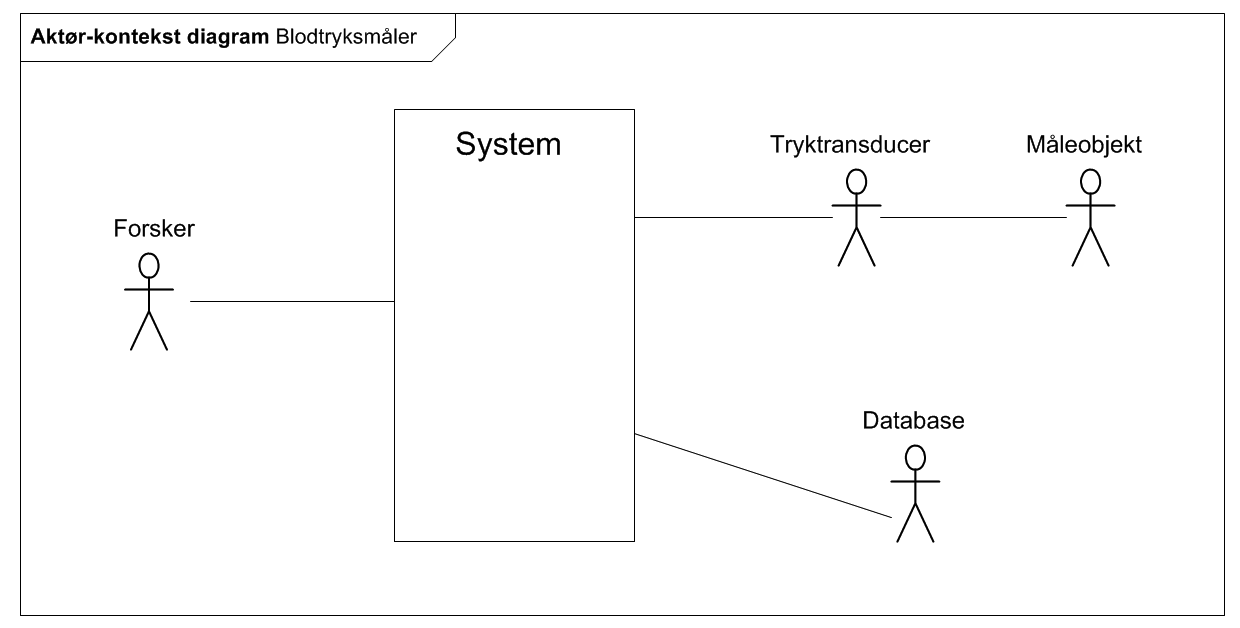
\includegraphics[width=1\textwidth]{Figurer/Snip20151104_43}
	\caption{Aktør-kontekstdiagram}
	\label{fig:aktoerbeskrivelse}
\end{figure}

Systemet består af en software- og en hardward-del. Softwaredelen er udarbejdet i Visual Studio C\#. Hardwaredelen består af flere komponenter sat sammen. Tryktransducer, Instrumentationforstærker, et aktivt 2. ordens lavpasfilter af typen Sallen-Key med unity gain og en DAQ. Det er selve systemet. \\
Primær aktøren i dette projekt er en Forsker. Sekundære aktører er Database, Tryktransducer og Måleobjekt. Måleobjekt er en package af Physionet og Analog Discovery, som er eksterne aktører.   

\subsection{Aktørbeskrivelse}

\begin{table}[H]
\begin{tabularx}{\textwidth}{l X}
     Aktørnavn & Forsker \\
     Type & Primær \\
     Beskrivelse  & Person med relevant baggrundsviden inden for blodtryksanalyse \\ 
     \midrule
     Aktørnavn & Tryktransducer \\
     Type & Sekundær \\
     Beskrivelse  & Tryktransducer måler og omformer trykket fra Måleobjekt til et analogt signal \\ 
     \midrule
     Aktørnavn & Måleobjekt  \\
     Type & Sekundær \\
     Beskrivelse  & Måleobjekt i det færdigudviklede produkt er et signal genereret enten in vitro eller in vivo. I prototypen er Måleobjekt en kombination af Physionet og Analog Discovery. Måleobjekt repræsenterer data fra Physionet leveret til blodtryksmålingssystemet igennem Analog Discovery \\
     \midrule
     Aktørnavn & Database \\
     Type & Sekundær \\
     Beskrivelse  & Database bruges i blodtryksmålingssystemet til at gemme data \\ 
     \midrule
     Atørnavn & Physionet \\
     Type & Ekstern  \\
     Beskrivelse  & Physionet er en ekstern database, som indeholder blodtrykssignalet fra forskellige patienter \\
     \midrule
     Aktørnavn & Analog Discovery  \\
     Type & Ekstern \\
     Beskrivelse  & Analog Discovery omdanner data fra Physionet til at analogt signal \\                                                                                                                                                                          
     \bottomrule                                                                                                                   
    \end{tabularx}
    \caption {Aktørbeskrivelse}
    \label{tab:aktoerbeskrivelse}
	
\end{table}

\subsection{Use case-diagram}
\begin{figure}[H]
	\centering
	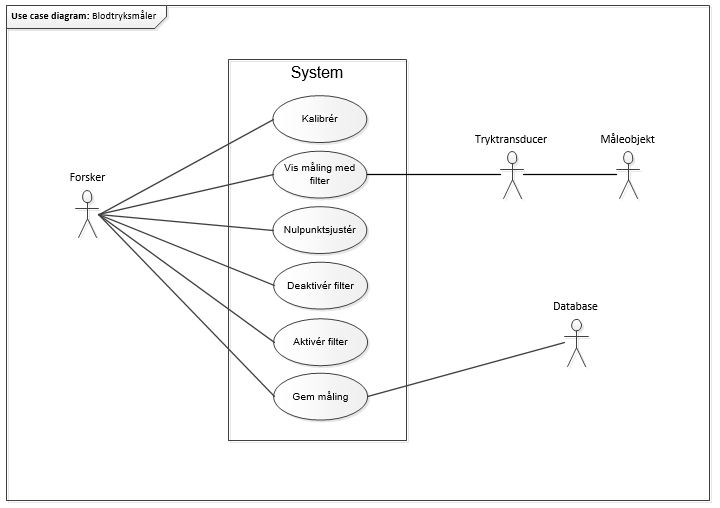
\includegraphics[width=1\textwidth]{Figurer/1}
	\caption{Use case-diagram}
	\label{fig:Use case-diagram}
\end{figure}

Forskeren af systemet er den primære aktør i alle seks Use Cases. Det er Forskeren, der sætter alle Use Cases igang og styrer, hvad der skal ske og hvornår. Tryktransducer, som er en af de sekundære aktører, interagerer i UC2. Tryktransduceren behandler tryk fra den anden sekundære aktør Måleobjekt, og omformer det til et analog signal. Blodtryksmålingen skal vises i UC2. For at få gemt data interagerer den sekundære aktør Database med UC6.  

\subsection{Use Cases}

\begin{longtabu} to \linewidth{@{}l r X[j]@{}} %UC1%
    {\large \textbf{Use Case 1}} && \\
    \toprule
    Navn &&    Kalibrér\\
    Use case ID &&    1\\
    Samtidige forløb &&    1\\
    Primær aktør &&    Forsker\\
    Sekundære aktør &&	 \\
    Mål &&    Forsker ønsker at kalibrere systemet\\
    Initiering &&	Startes af Forsker\\
    Forudsætninger &&  System er aktivt og tilgængeligt\\
    Resultat &&		System er kalibreret                         \\ \midrule
    Hovedforløb &    1. &	 Kalibrering-vinduet vises ved opstart og 					tidligere kalibreringsdata vises\\[-1ex]  
    			&	 2. &	 Forsker indtaster målte kalibreringsdata    			\newline
    						 [2.a \textit{Forsker vælger ikke at kalibrere}]\newline
    						 [2.b \textit{Indtastede kalibreringsdata er ugyldige}]\\
                &    3.	&	 System kalibrerer\\
                &	 4. &	 Det fremgår i Kalibrering-vinduet, at kalibrering er udført \newline\\ \midrule
                
    Undtagelser &    2.a &   Forsker ønsker ingen kalibrering. UC1 afsluttes og Kalibrering-vinduet lukkes  \\
    			&	 2.b &	 Det fremgår i Kalibrering-vinduet, at indtastede kalibreringsdata er ugyldige. Forsætter ved UC1 punkt 2  \\ \bottomrule
\caption{Fully dressed Use Case 1.}
\label{UC1}
\end{longtabu}


\begin{longtabu} to \linewidth{@{}l r X[j]@{}} %UC2%
    {\large \textbf{Use Case 2}} && \\
    \toprule
    Navn &&    Vis Måling med digitalt filter\\
    Use case ID &&    2\\
    Samtidige forløb &&    1\\
    Primær aktør &&    Forsker\\
    Sekundære aktør &&	 Måleobjekt og Tryktransducer\\
    Mål &&    Forsker ønsker at vise blodtrykssignal med digitalt filter\\
    Initiering &&	Startes efter afsluttet UC1\\
    Forudsætninger &&  System er aktivt og tilgængeligt. Digitalt filter er aktivt. Tryktransducer er tilsluttet system. Måleobjekt er tilsluttet tryktransducer\\
    Resultat &&		Det filtrerede blodtrykssignal udskrives                         \\ \midrule
    Hovedforløb &    1. &    Det filtrerede blodtrykssignal vises i en graf i Monitor-vinduet\newline\\ \midrule
                
    Undtagelser &    &   \\ \bottomrule
\caption{Fully dressed Use Case 2.}
\label{UC2}
\end{longtabu}


\begin{longtabu} to \linewidth{@{}l r X[j]@{}} %UC3%
    {\large \textbf{Use Case 3}} && \\
    \toprule
    Navn &&    Nulpunktsjustér\\
    Use case ID &&    3\\
    Samtidige forløb &&    1\\
    Primær aktør &&    Forsker\\
    Sekundære aktør && \\
    Mål &&    Forsker ønsker at nulpunktsjustere system\\
    Initiering &&	Startes af Forsker\\
    Forudsætninger &&  System er aktivt og tilgængeligt. UC2 kører. Tryktransduceren skal befinde sig i atmosfærisk luft  \\    
    Resultat &&		System er nulpunktsjusteret\\ \midrule
    Hovedforløb &    1. &    Forsker vælger at udføre en nulpunktsjustering\\[-1ex]   						 	
                &    2. &    System nulpunktsjusterer\\[-1ex]
                &	 3.	&	 Det fremgår i Monitor-vinduet, at nulpunktsjustering er udført\newline\\ \midrule
                
    Undtagelser &     &      \\ \bottomrule
\caption{Fully dressed Use Case 3.}
\label{UC3}
\end{longtabu}

\begin{longtabu} to \linewidth{@{}l r X[j]@{}} %UC4%
    {\large \textbf{Use Case 4}} && \\
    \toprule
    Navn &&    Deaktivér filter\\
    Use case ID &&    4\\
    Samtidige forløb &&   1\\
    Primær aktør &&    Forsker\\
    Sekundære aktør &&	 \\
    Mål &&    Forsker ønsker at deaktivere det digitale filter\\
    Initiering &&	Startes af Forsker\\
    Forudsætninger &&  System er aktivt og tilgængeligt. UC2 kører  \\
    Resultat &&		Ufiltreret blodtrykssignal vises i Monitor-vinduet                 \\ \midrule
    Hovedforløb &    1. &    Forsker vælger at deaktivere digitalt filter \\[-1ex]   						 	
                &    2. &    System udskriver det ufiltrerede blodtryksignal\newline\\ \midrule
                
    Undtagelser &     &      \\ \bottomrule
\caption{Fully dressed Use Case 4.}
\label{UC4}
\end{longtabu}


\begin{longtabu} to \linewidth{@{}l r X[j]@{}} %UC5%
    {\large \textbf{Use Case 5}} && \\
    \toprule
    Navn &&    Aktivér filter\\
    Use case ID &&    5\\
    Samtidige forløb &&   1\\
    Primær aktør &&    Forsker\\
    Sekundære aktør &&	 \\
    Mål &&    Forsker ønsker at aktivere det digitale filter\\
    Initiering &&	Startes af Forsker\\
    Forudsætninger &&  System er aktivt og tilgængeligt. UC4 er afsluttet  \\
    Resultat &&		Filtreret blodtrykssignal vises i Monitor-vindet                 \\ \midrule
    Hovedforløb &    1. &    Forsker vælger at aktivere digitalt filter\\[-1ex]   						 	
                &    2. &    System udskriver det filtrerede blodtrykssignal\newline\\ \midrule
                
    Undtagelser &     &      \\ \bottomrule
\caption{Fully dressed Use Case 5.}
\label{UC5}
\end{longtabu}
    
\begin{longtabu} to \linewidth{@{}l r X[j]@{}} %UC6%
    {\large \textbf{Use Case 6}} && \\
    \toprule
    Navn &&    Gem måling\\
    Use case ID &&    6\\
    Samtidige forløb &&   1...*\\
    Primær aktør &&    Forsker\\
    Sekundære aktør &&	Database\\
    Mål &&    Forsker ønsker at gemme data i Database\\
    Initiering &&	Startes af Forsker\\
    Forudsætninger &&  System er aktivt og tilgængeligt. UC4 eller UC5 kører  \\
    Resultat &&		Data er gemt i Database                 \\ \midrule
    Hovedforløb &    1. &    Forsker bestemmer optagelseslængde for målingen i Monitorvindue \newline
    						 [1.a \textit{Forsker ændrer ikke optagelseslængden for målingen}]\\   						 
                &    2. &    Forsker igangsætter optagelse af målingen 		 \\[-1ex] 
                &    3.	&	 Målingen stopper\newline
                			 [3.a \textit{Forsker stopper optagelsen af måling inden optagelseslængden er nået}]\\
                &	 4.	&	 Forsker åbner Gem-vinduet\\[-1ex]			 
                &	 5. &	 Forsker indtaster oplysninger om målingen \\[-1ex]
                &	 6. &	 Forsker trykker på "OK"\--knappen og system gemmer målingen i Database				 \\[-1ex]
                &	 7.	&	 Det fremgår af 	Gem-vinduet, at målingen 		 er gemt\newline\\ \midrule
                
    Undtagelser &    1.a &   Forsker ønsker ikke at ændre optagelseslængde for målingen. Forsætter ved punkt 2 i UC6 \\
      			&    3.a &   Forsker stopper optagelse af målingen. Forsætter ved punkt 4 i UC6  \\
\bottomrule
    
\caption{Fully dressed Use Case 6.}
\label{UC6}
\end{longtabu}

\section{Ikke-funktionelle krav}
De ikke-funktionelle krav er specificeret ved brug af redskabet (F)URPS+, der står for hhv. Functionality, Usability, Reliability, Performance, Supportability og andre krav til fx brugssituationer og interface.  


\subsection{Functionality}
\begin{itemize}
	\item System skal kunne kalibreres. 
	\item System skal kunne vise et kontinuert blodtrykssignal i Monitor-vinduet.
	\item System skal kunne vise systole-, diastole- og pulsværdier med op til tre cifre.
	\item System skal kunne vise et blodtrykssignal med og uden et digitalt filter.
	\item System skal kunne nulpunktsjustere blodtrykssignalet.
	\item System skal kunne gemme en blodtryksmåling i en database.
\end{itemize}

\subsection{Usability}
\begin{itemize}
	\item Kalibrering-vinduet skal indeholde tekstbokse til indtastning af kalibreringsdata. 
	\item Kalibrering-vinduet skal indeholde en "Beregn"\--knap. 
	\item Kalibrering-vinduet skal indeholde en "OK"\--knap.
	\item Kalibrering-vinduet skal indeholde et tidsstempel for seneste kalibrering.
	\item Monitor-vinduet skal indeholde en ”Gem”\--knap.
	\item Monitor-vinduet skal indeholde en ”Nulpunktsjustér”\--knap.
	\item Monitor-vinduet skal indeholde et tidsstempel for seneste nulpunktsjustering.
	\item Monitor-vinduet skal indeholde to radiobuttons til aktivering og deaktivering af digitalt filter.
	\item Monitor-vinduet skal indeholde en tekstboks til ændring af optagelseslængden.  
	\item Monitor-vinduet skal indeholde en "Rec"\--knap/.
	\item Monitor-vinduet skal indeholde en "Stop"\--knap.
	\item Gem-vinduet skal indeholde tekstbokse til indtastning af oplysninger om målingen. 
	\item Gem-vinduet skal indeholde en ”OK”\--knap.
	\item Det skal være muligt at aflæse systole-, diastole- og pulsværdier på Monitor-vinduet fra 2 meters afstand med normalt syn.
\end{itemize}

\subsection{Reliability}
\begin{itemize}
	\item Systemet skal have en effektiv MTBF (Mean Time Between Failure) på 99 timer og en MTTR (Mean Time To Restore) på 20 minutter (1/3 time).
				\begin{align}
					Availability = \frac{MTBF}{MTBF+MTTR} = \frac{99}{99+1/3} = 0,997 = 99,7 \%
				\end{align}

\end{itemize}

\subsection{Performance}
\begin{itemize}
	\item Blodtrykssignalet skal vises maksimalt 5 sekunder efter UC1 er afsluttet.
	\item Systemet skal vise en graf for blodtryksmålingen, hvor y-aksen er mmHg og x-aksen er tid i sekunder.
	\item Systemet skal kunne måle blodtryksværdier fra 0 til 300 mmHg.
	\item Blodtrykssignalet vises kontinuerligt over et interval af fire sekunder af gangen.
	\item Blodtrykssignalet vises via en rød kurve. 
	\item Y-aksen varierer efter blodtrykssignalets maksimum- og minimumværdier.  
\end{itemize}

\subsection{Supportability}
\begin{itemize}
	\item Softwaren skal opbygges efter trelagsmodellen.
\end{itemize}

\subsection{Andre(+)}
\textbf{Brugssituationer}
\begin{itemize}
	\item Der skal være adgang til en computer med Windows 7 eller nyere – computeren skal have minimum 4 GB RAM.
	\item Der skal være adgang til en computer, hvor National Instruments er installeret.
\end{itemize}
\textbf{Interface}
\begin{itemize}
	\item Blodtryksdiagrammet skal fylde minimum 1/3 af Monitor-vinduet.
	\item Baggrunden i Monitor-vinduet skal være mørk.
	\item Blodtrykssignal og -værdier(systole og diastole) skal være røde, og puls skal være grøn.
	\item Systolisk og diastolisk blodtryk skal fremhæves øverst i højre hjørne ved større skriftstørrelse end andre værdier i Monitor-vinduet (fx værdier på akserne).
\end{itemize}













